\documentclass[12pt]{article}
\usepackage[margin=1in]{geometry}
\usepackage{setspace}
\usepackage{graphicx}
\usepackage{booktabs}
\usepackage{amsmath}
\usepackage{natbib}
\usepackage{caption}
\usepackage[hidelinks]{hyperref}
\usepackage{microtype}
\bibliographystyle{plainnat}
\captionsetup{font=small,labelfont=bf}
\graphicspath{{../output/figures/}}

\title{\bf Prevention Without Proof}
\author{Scott Cunningham\\ \small Baylor University}
\date{\small Prepared for the European Commission, Joint Research Centre, Ispra \\ \small June 2026}

\begin{document}
\maketitle
\thispagestyle{empty}

\begin{abstract}
\noindent
For two decades the world's governments have answered suicide with strategy
documents, and for two decades we have told ourselves they work. They may. But the
cross-national record cannot show it. Re-examining the staggered adoption of national
suicide-prevention strategies across Europe with estimators robust to treatment-effect
heterogeneity, I find that suicide rises, not falls, after adoption---by roughly three
deaths per hundred thousand. Measured correctly, parallel trends hold; but with four
treated countries that is no comfort. The estimate cannot be signed, a placebo cannot
distinguish it from chance, and it halves when the comparison group changes. We are
governing mortality on faith.
\end{abstract}

\vfill
\begin{center}
\small JEL: I18, I12, C23. \quad Keywords: suicide; difference-in-differences; staggered adoption;
parallel trends; mental health policy.
\end{center}
\clearpage

\doublespacing
\setcounter{page}{1}

\section{Introduction}

Every forty seconds, somewhere on earth, a person decides that the rest of life is not worth
the rest of life. The decision is private, but its accounting is public: more than seven hundred
thousand such deaths a year, more than war, more than homicide, more than most of the diseases we
have organized entire ministries to defeat. Confronted with a number this large and this stubborn,
governments have done what governments do. They have written strategies. Since the early 1990s a
national suicide-prevention strategy has gone from a Nordic experiment to an article of
international faith: the World Health Organization now urges every member state to adopt one, and
dozens have \citep{who2014preventing,who2018strategies}. We have decided, collectively, that the
document is the cure.

This paper asks the question that the strategies themselves were supposed to answer and never
did. Do they work? Not in the sense of whether they are well-meant---they are---or whether they
contain sensible ideas---they do---but in the only sense that matters to the person standing on
the bridge: does a country that adopts a national suicide-prevention strategy bury fewer of its
citizens afterward than it otherwise would have? The question is empirical, it is answerable in
principle, and it is, I will argue, almost entirely unanswered in practice. We have spent twenty
years and an enormous reserve of moral capital on an intervention whose effect on the outcome it
names we cannot, from the cross-national record, distinguish from zero, from harm, or from
salvation.

That is an uncomfortable thing to say in a building full of people whose job is to prevent
suicide, so let me be precise about what I am and am not claiming. I am not claiming that
suicide-prevention strategies fail. I am claiming something narrower and, I think, more
disturbing: that the research design which the field has relied upon to conclude that they
succeed does not survive contact with the methods we now know are necessary when policies are
adopted at different times by different places \citep{goodmanbacon2021did,roth2023trending}. The
canonical finding---that countries with strategies see suicide fall relative to countries
without them \citep{matsubayashi2011effect}---rests on a two-way fixed-effects comparison that,
under staggered adoption and heterogeneous effects, can return the wrong sign for mechanical
reasons that have nothing to do with the policy. When I re-estimate the same kind of comparison
on real European data with the heterogeneity-robust tools of
\citet{callaway2021did}, \citet{borusyak2024revisiting}, and \citet{sun2021estimating}, the
protective effect does not merely shrink. It reverses. And then, under honest scrutiny, it
dissolves.

The reversal is instructive precisely because it is not real. Suicide is higher after a country
adopts a strategy than a naive comparison with non-adopters would predict---by about three deaths
per hundred thousand, an estimate that three different modern estimators agree on to within a
fraction of a death. It is tempting to reach for the obvious explanation---that suicide was rising
in these countries before they adopted---but when the pre-adoption trends are measured correctly,
as long differences from the year before treatment, they are flat: the data do not support a story
of differential pre-trends. The confound is subtler and harder to dismiss. The post-adoption rise
loads on calendar years 2008 through 2010---the Great Recession, the most violent macroeconomic
shock to European mental health in a generation, and one the suicide literature has already shown
raises the toll \citep{reeves2012increase,stuckler2013body}. The later-adopting treated countries
spent their entire post-period inside that shock. The positive ``effect'' is, in part, the residue
of when prevention's first years happen to fall---and, as I will show, an estimate too weak and too
fragile to carry any weight at all.

None of this would be worth a paper if the only casualty were a single optimistic estimate. The
casualty is larger. It is the idea that we can read the worth of a suicide-prevention strategy off
the cross-national mortality record at all. I show that the parallel-trends assumption on which
every such reading depends cannot be \emph{rejected}---but only because four treated countries
cannot test it with any power; that the propensity to adopt is so perfectly predicted by a
country's characteristics that there is no overlap to lean on; that the sensitivity analysis of
\citet{rambachan2023credible} cannot sign the post-adoption effect under even mild departures from
parallel trends; and that a synthetic-control comparison,
the method designed for exactly this scarcity of treated units, produces gaps statistically
indistinguishable from placebos drawn at random. These diagnostics are not independent of one
another---the sensitivity analysis formalizes the pre-trend, and the placebo and the synthetic
control are both, at bottom, statements about how little a handful of treated countries can tell
us---but they are different windows onto the same wall, and through every one of them the answer is
the same word: undetermined.

I do not regard this as a nihilistic result, and I will end by explaining why. A finding that the
evidence cannot bear the weight we have placed on it is not the same as a finding that the policy
is worthless; it is a finding that we have been navigating in the dark and calling it sight. The
moral content of that statement is not small. We owe the people these strategies are meant to save
an honest account of whether they are saved, and we do not have one. The remainder of this paper
is the attempt to say exactly how much we do not have, and why, and what it would take to know
more.

\section{A Policy Adopted in the Dark}

The modern national suicide-prevention strategy was born in Finland. Between 1986 and 1992 the
Finns did something no country had done: they investigated every suicide in the nation for a year,
built a prevention program on what they learned, and made suicide reduction an explicit object of
national policy. The Finnish suicide rate, then among the highest in the world, fell. Whether it
fell \emph{because} of the program or because it had nowhere to go but down from a historic peak is
a question the Finnish experience alone cannot answer, and that ambiguity---the impossibility of
separating the policy from the conditions that produced it---is the theme of everything that
follows.

What Finland began, the world copied. Norway published a strategy in 1995, Sweden built a program
the same year, France launched a five-year national plan in 2000, England and Scotland adopted
strategies in 2002, Ireland in 2005. By 2018 the WHO could count dozens of national strategies and
could exhort the rest \citep{who2018strategies}. The diffusion was rapid, it was sincere, and it
was almost entirely uninformed by credible evidence that the thing being diffused did what it
promised. The single most cited piece of evaluation, \citet{matsubayashi2011effect}, compared
suicide rates in eleven OECD countries that had adopted national programs against ten that had not,
and reported reductions concentrated among the young and the old. It was a careful paper for its
time. Its time was before we understood what two-way fixed effects do to staggered treatments.

We understand now. When units adopt a treatment at different dates and the treatment's effect
differs across units or evolves over time, the two-way fixed-effects estimator does not recover a
sensible average of those effects. It recovers a weighted combination in which already-treated
units serve as controls for newly-treated ones, the weights can be negative, and the resulting
number can lie outside the range of every true effect it is meant to summarize
\citep{goodmanbacon2021did,dechaisemartin2020twoway}. The profession has spent five years building
estimators that avoid this trap \citep{callaway2021did,sun2021estimating,borusyak2024revisiting},
and a parallel literature on how to probe the assumption---parallel trends---on which all of them
still depend \citep{rambachan2023credible,roth2023trending}. The suicide-prevention literature has
not caught up. This paper is, in part, an attempt to make it.

\section{Data}

I assemble a country-by-year panel of European suicide mortality from three real, public sources;
nothing here is simulated. The outcome is the age-standardized suicide rate---deaths from
intentional self-harm (ICD-10 codes X60--X84 and Y87.0) per hundred thousand population---published
by Eurostat for the years 1994 through 2010 \citep{eurostat_cod}. The treatment is the year, if
any, in which a country's government adopted a stand-alone national suicide-prevention strategy,
coded from the WHO's 2018 inventory \citep{who2018strategies} and cross-checked against the
peer-reviewed adoption dates of \citet{lewitzka2019national}; Appendix~A documents every country's
coding and its source. The single time-varying covariate is the national unemployment rate from the
World Bank's modeled ILO series \citep{worldbank_unemp}, included because the business cycle is the
best-established time-varying determinant of suicide we possess \citep{ruhm2000recessions,
reeves2012increase}.

Three features of the data govern everything that can and cannot be learned from it. First, the
Eurostat regional series begins only in 2011, so the long pre-adoption history needed to test
parallel trends exists only at the national level, which is where I work. Second, the window
1994--2010 brackets the main European adoption wave but starts too late for the earliest adopters:
Finland (1992) is already treated when the data begin and is dropped, and France (2000) is dropped
because its suicide series does not begin until 2001, leaving it no pre-period. Third, and most
consequentially, the number of treated countries with a usable pre-period is small---four. Norway
and Sweden adopt in 1995, the United Kingdom in 2002, Ireland in 2005. Against them stand twelve
countries that the WHO documents as never having adopted a stand-alone national strategy in the
window---Germany, Italy, Spain, Belgium, Austria, Switzerland, the Netherlands, Portugal, Greece,
Luxembourg, Czechia, Estonia, Hungary, Slovenia. The balanced panel retains the twelve of these
with a complete suicide and unemployment record over 1994--2010---Austria, Switzerland, Czechia,
Germany, Estonia, Greece, Spain, Hungary, Luxembourg, the Netherlands, Portugal, Slovenia---while
Belgium, Denmark, Poland, Slovakia, and Italy are dropped for gaps in the suicide series. Italy's
exclusion deserves a word, because Italy is the country in which these words are being read. Its
suicide series is missing 2004 and 2005, so it cannot enter the balanced estimand; but Italy is a
documented never-adopter, a large European nation that never wrote the document, and it remains the
natural backdrop to everything that follows---the silent control against which the writers of
strategies might have been judged, had the data let us judge them.

Four treated units is not a defect of my execution; it is the size of the natural experiment.
\citet{matsubayashi2011effect} had eleven. The European cross-section is simply not large, the
adoption dates are clustered, and the data begin late. I will not pretend otherwise, and the
reader should hold the smallness of the treated group in mind through every estimate that follows,
because it is the reason the honest conclusion is one of uncertainty rather than refutation.

A word on inference follows from the same smallness. With four treated countries and twelve
controls the panel has on the order of sixteen clusters, far too few for the cluster-robust and
multiplier-bootstrap standard errors the estimators report by default to be believed; I report
them because convention demands it, but I do not lean on them, and neither should the reader.
The inferential weight is carried instead by randomization inference---the in-space placebo of
Section~6, which asks how often a fake adoption assigned at random among the never-treated produces
an estimate as large as the one we observe. That frequency, not a $t$-statistic, is the honest
measure of how surprised we should be.

\section{Design: What We Are Trying to Measure}

\paragraph{The estimand.} I target the average effect of having adopted a strategy on suicide in
the countries that adopted one---the average treatment effect on the treated, aggregated across
adoption cohorts with weights proportional to the number of treated countries in each cohort. This
is the group-size-weighted summary of the group-time average treatment effects $ATT(g,t)$ of
\citet{callaway2021did}: for each cohort $g$ and year $t$ it compares the change in suicide from
just before $g$'s adoption to year $t$, in cohort $g$ versus countries not yet (or never) treated,
and then averages. I report the simple equally-weighted average as well; the two differ only in how
much weight the long-observed 1995 cohort receives.

\paragraph{The identifying assumption and the covariate.} Identification rests on conditional
parallel trends: absent adoption, suicide in treated and comparison countries would have evolved in
parallel, possibly after conditioning on covariates. The covariate I condition on is unemployment,
and the choice is deliberate. If one asks what an expert on suicide would insist be held fixed
before attributing a mortality change to a policy, the answer is the economy: recessions raise
suicide, recoveries lower it, and the timing of Europe's recessions is not independent of the
timing of its prevention strategies \citep{ruhm2000recessions,stuckler2009publichealth,
reeves2012increase}. Aging and income matter too, but they move slowly and are absorbed by the
country and year structure; unemployment is the fast-moving confounder that can masquerade as a
treatment effect, and it is the one I take most seriously.

\paragraph{Why regression adjustment and not weighting.} A doubly robust or inverse-propensity
estimator would, in principle, be preferable. It is not available here in any honest form. When I
estimate the probability that a country ever adopts a strategy as a function of its baseline
characteristics, the model separates the data perfectly: every treated country receives a
predicted probability indistinguishable from one and every control a probability indistinguishable
from zero (Figure~\ref{fig:pscore}). There is no region of common support in which a propensity
score could reweight anything; to use one would be to extrapolate off functional form and call it
identification. I therefore use the regression-adjustment form of the
\citet{callaway2021did} estimator, which models the conditional evolution of the outcome rather
than the probability of treatment, and I report the doubly robust and inverse-propensity variants
only to show that they change nothing of substance.

\begin{figure}[t]
\centering
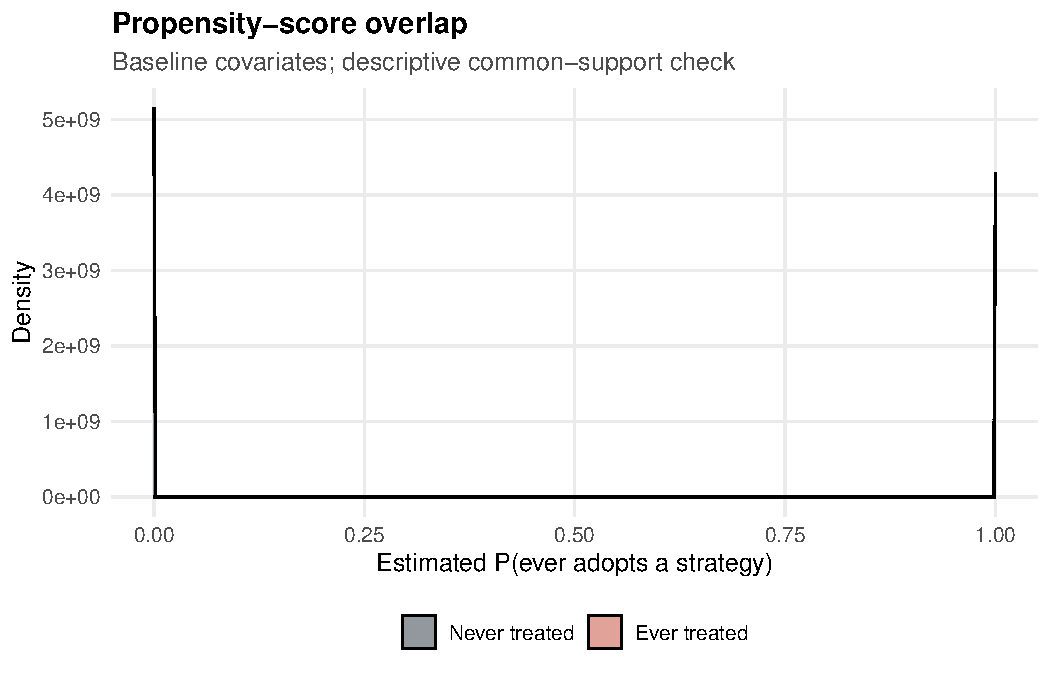
\includegraphics[width=0.75\textwidth]{fig3_pscore_overlap.pdf}
\caption{Propensity-score overlap fails by construction. A country-level logit of ever-adoption on
baseline covariates separates the four treated countries (scores $\approx 1$) from the twelve
controls (scores $\approx 0$) perfectly. With no common support, propensity weighting is
inappropriate; the analysis uses regression adjustment.}
\label{fig:pscore}
\end{figure}

\paragraph{The rollout.} Figure~\ref{fig:rollout} shows the staggered adoption that identifies the
design, and Figure~\ref{fig:cohorts} the cohort sizes. The picture is honest about its own
thinness: two countries enter treatment in 1995, one in 2002, one in 2005, against a wall of
never-treated grey.

\begin{figure}[t]
\centering
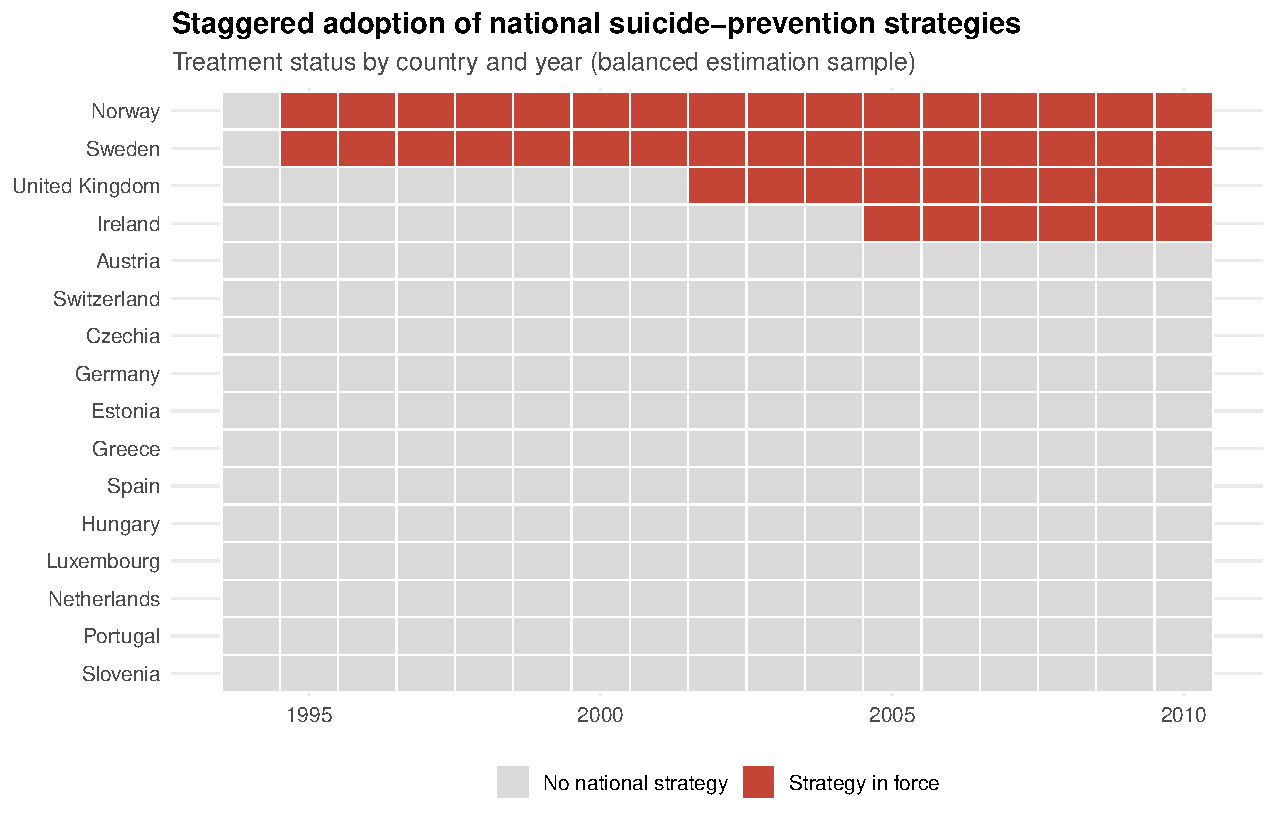
\includegraphics[width=0.85\textwidth]{fig4_panelview.pdf}
\caption{Staggered adoption of national suicide-prevention strategies, balanced estimation sample,
1994--2010. Red indicates a strategy in force.}
\label{fig:rollout}
\end{figure}

\begin{figure}[t]
\centering
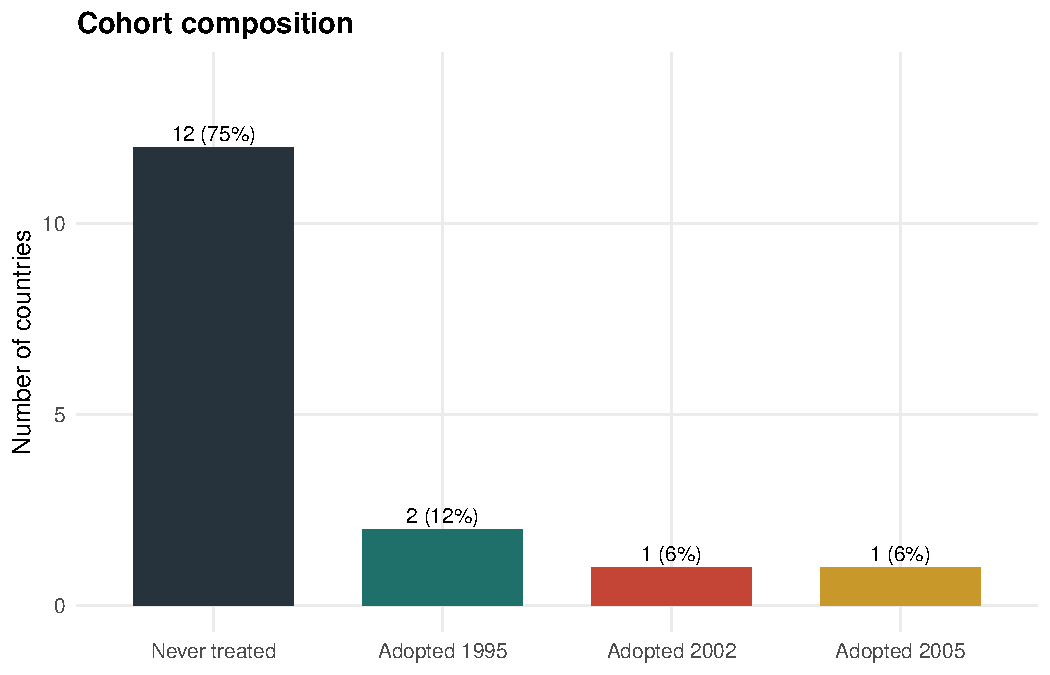
\includegraphics[width=0.62\textwidth]{fig5_cohort_counts.pdf}
\caption{Cohort composition. Twelve never-treated controls; four treated countries in three
adoption cohorts.}
\label{fig:cohorts}
\end{figure}

\section{What the Data Say}

Before any model, look at the outcome. Figure~\ref{fig:bycohort} plots mean suicide by adoption
cohort. Two things are visible to the naked eye. The treated countries do not look like the
controls---they start lower---which is why levels comparisons are useless and why we need the
within-country, difference-in-differences logic at all. And the lines bend upward together at the
right edge, in the recession years, treated and untreated alike.

\begin{figure}[t]
\centering
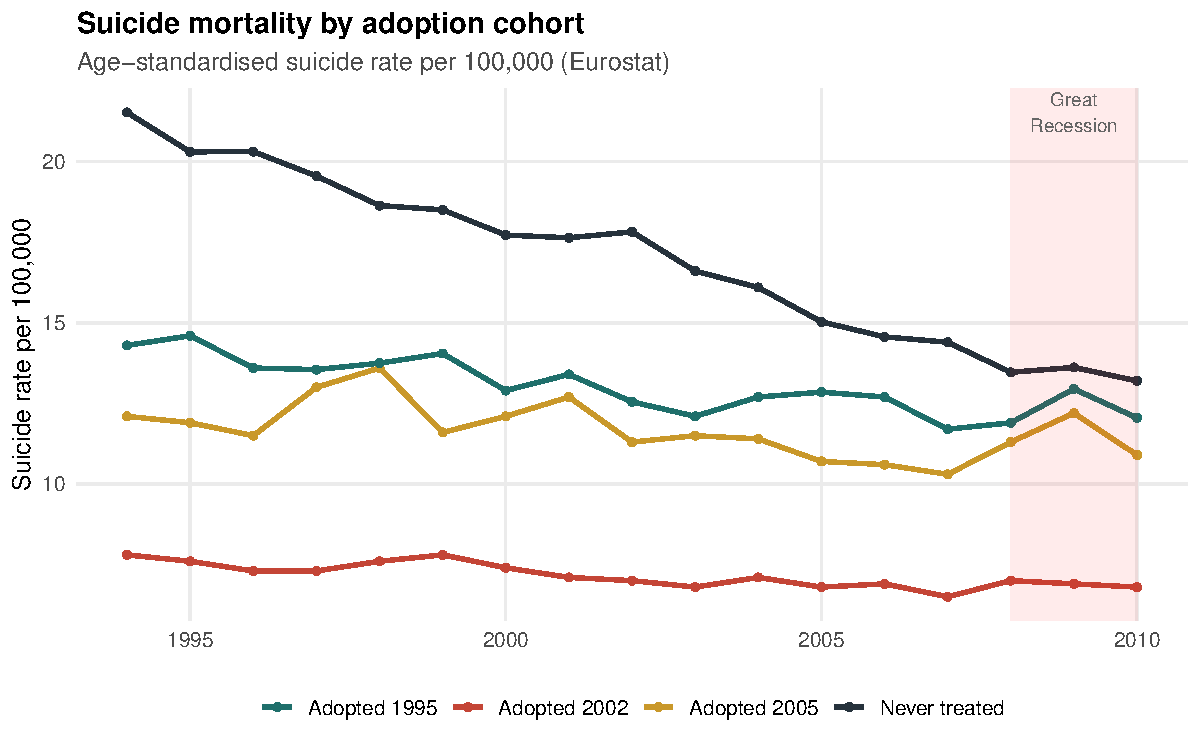
\includegraphics[width=0.85\textwidth]{fig6_outcome_by_cohort.pdf}
\caption{Suicide mortality by adoption cohort. The shaded band marks the 2008--2010 recession.}
\label{fig:bycohort}
\end{figure}

The headline estimate is positive. Conditioning on unemployment and using never-treated countries
as the comparison group, the group-size-weighted average treatment effect on the treated is
$+2.73$ suicides per hundred thousand (standard error $1.05$); the simple average is $+3.05$
($1.24$). The sign is robust to estimation choices that ought to matter and do not:
Table~\ref{tab:estimators} collects the doubly robust variant ($+2.56$), the unconditional variant
($+2.76$), the not-yet-treated comparison group ($+2.66$), the imputation estimator of
\citet{borusyak2024revisiting} ($+3.23$), and the interaction-weighted estimator of
\citet{sun2021estimating} ($+3.03$). Three families of heterogeneity-robust estimators, built on
different assumptions, agree that suicide is higher after adoption by something close to three
deaths per hundred thousand. Figure~\ref{fig:overlay} shows their event-study paths lying almost on
top of one another.

\begin{table}[t]
\centering\small
\caption{The estimate is positive and robust to estimator choice}
\label{tab:estimators}
\begin{tabular}{lcc}
\toprule
Estimator / specification & ATT (per 100{,}000) & SE \\
\midrule
Callaway--Sant'Anna, reg., +unemployment (\emph{primary}) & $+2.73$ & $1.05$ \\
\quad simple average & $+3.05$ & $1.24$ \\
\quad doubly robust & $+2.56$ & --- \\
\quad unconditional & $+2.76$ & --- \\
\quad not-yet-treated comparison & $+2.66$ & --- \\
Borusyak--Jaravel--Spiess (imputation) & $+3.23$ & $1.30$ \\
Sun--Abraham (interaction-weighted) & $+3.03$ & $1.38$ \\
\bottomrule
\end{tabular}
\end{table}

\begin{figure}[t]
\centering
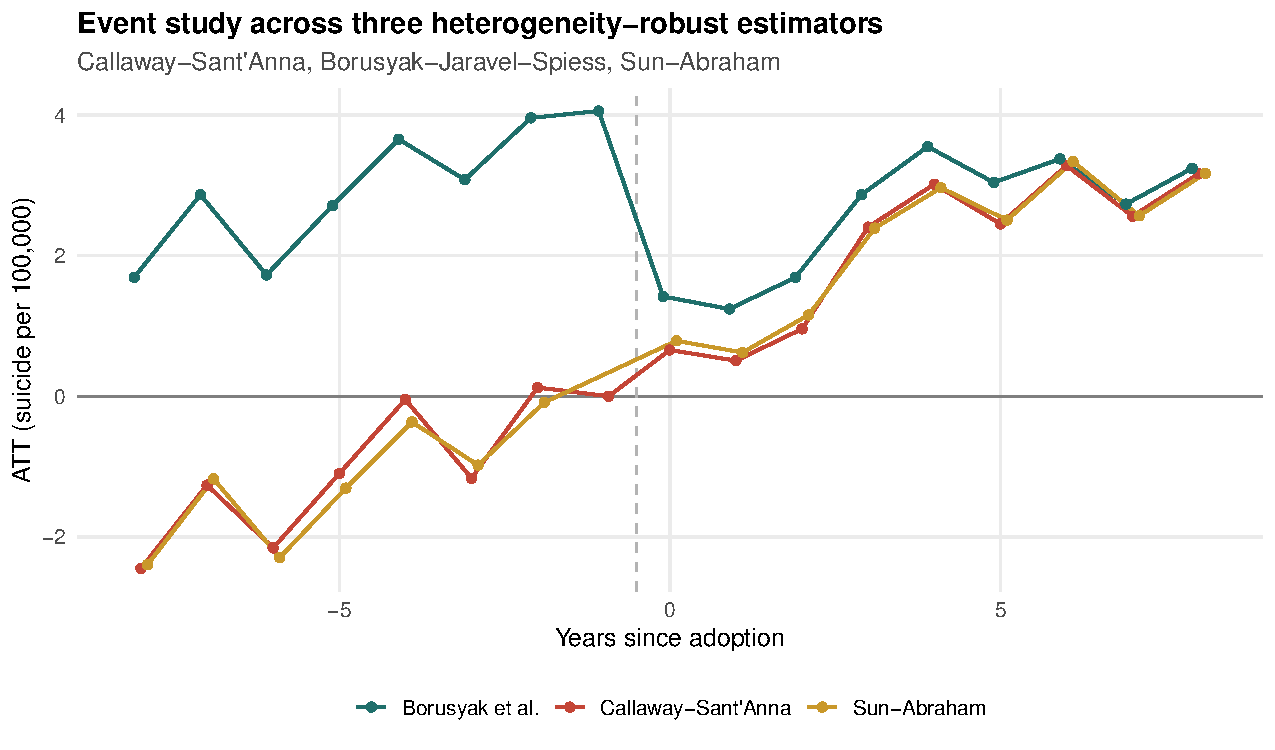
\includegraphics[width=0.9\textwidth]{fig_robust_overlay.pdf}
\caption{Event studies from three heterogeneity-robust estimators. The estimators agree.}
\label{fig:overlay}
\end{figure}

A reader who stopped here would conclude that suicide-prevention strategies are followed by more
suicide, and a careless reader might even write the headline. The reader should not stop here.
Everything from this point forward is the argument that this number, however robust to the choices
econometricians usually worry about, measures something other than the effect of the policy.

\section{What the Number Is Not}

\paragraph{It survives the pre-trend test---but the test is nearly blind.} The event study in
Figure~\ref{fig:event} plots the Callaway--Sant'Anna effect by years since adoption, with every
coefficient---before and after---a long difference from the year just before treatment, the same
$g-1$ baseline against which the post-adoption effects and the parallel-trends assumption itself are
defined. Look left of zero. The pre-adoption coefficients are negative and noisy, and jointly they
do not reject a flat path: the sum of squared $t$-statistics across the eight pre-periods is
$9.9$, comfortably inside what chance produces on eight degrees of freedom. Measured the right way,
parallel trends cannot be rejected. I want to be exact about what that does and does not buy. It
removes the most common objection to a result like this---that the treated countries were already
diverging---but it removes it the way an unlit room removes the objection that the furniture is
ugly. With four treated countries the pre-trend test is powered to catch only gross violations; its
silence is the silence of a design too small to hear anything, not a clean bill of health. (An
earlier draft, using the short, period-to-period baseline that much applied work still reports,
found a large spurious violation. The long-difference baseline is the correct one, and it is flat;
the lesson that the choice of baseline can manufacture or erase a pre-trend is not the smallest one
in this paper.)

The little the test can see, it sees through two countries. The pre-adoption leads are identified
almost entirely off the United Kingdom and Ireland; Norway and Sweden, adopting in 1995 with a
single pre-period each, contribute to the \emph{level} of the effect but nothing to the \emph{test}
of trends. The estimand leans hardest on the cohort that cannot be checked at all.

\begin{figure}[t]
\centering
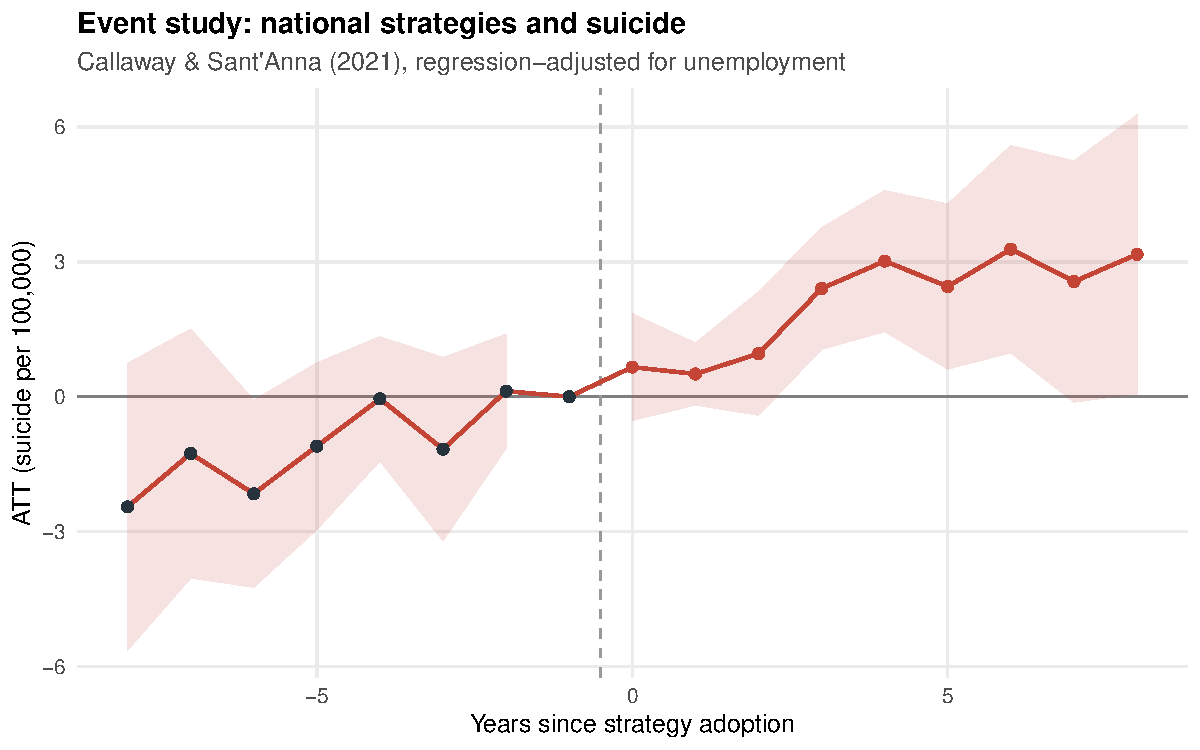
\includegraphics[width=0.85\textwidth]{fig8_event_study.pdf}
\caption{Event study, Callaway--Sant'Anna, universal (long-difference) baseline. Pre-adoption
coefficients (dark) do not jointly reject parallel trends ($\sum z^2 = 9.9$, 8 d.f.); the
post-adoption path is positive.}
\label{fig:event}
\end{figure}

\paragraph{It is not free of the recession.} Figure~\ref{fig:calendar} re-aggregates the same
group-time effects by calendar year rather than by event time. The estimated ``effect'' is small
or negative through the mid-2000s and then leaps upward in 2008 and stays there. The treated
cohorts' post-adoption windows---Ireland's especially, beginning in 2005---overlap precisely the
years in which austerity and unemployment drove European suicide up
\citep{reeves2012increase,stuckler2013body}. A staggered design cannot tell the effect of a 2005
policy apart from the effect of a 2008 recession that strikes the 2005 adopter during its
post-period. The positive ATT may be, in substantial part, the recession wearing the policy's
clothes; it may be selection; it may be noise. I do not claim to know which, and the claim is not
that the recession explains the result---to assert that would be to identify, from the same panel I
have just called uninformative, an effect I have no business identifying. The claim is the weaker
and more durable one: that these two forces are present, that the design cannot separate them from
the policy, and that a number which confounds all three is not a measurement of any one.

\begin{figure}[t]
\centering
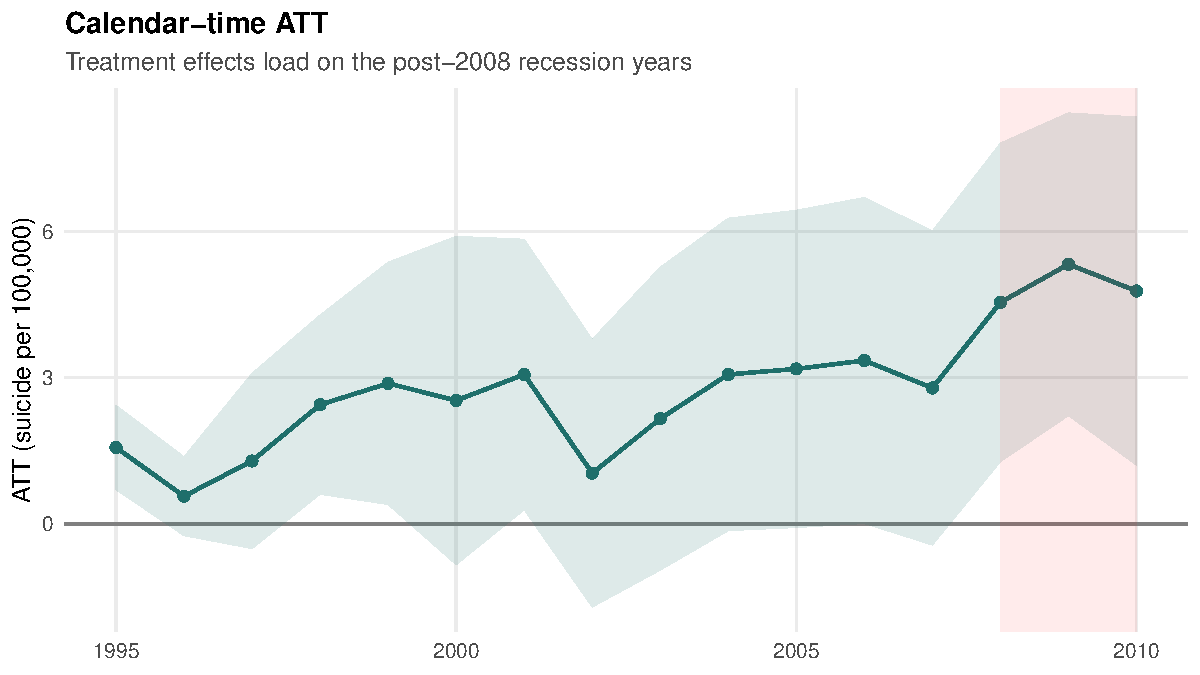
\includegraphics[width=0.85\textwidth]{fig8c_calendar.pdf}
\caption{Calendar-time aggregation. The ``effect'' materializes in 2008--2010, the recession years.}
\label{fig:calendar}
\end{figure}

\paragraph{It cannot be signed.} A pre-trend test that cannot reject is not the same as a
parallel-trends assumption that holds; the honest question is how robust the estimate is to the
violations the test is too weak to rule out. The sensitivity analysis of
\citet{rambachan2023credible} answers it: allowing post-adoption deviations from parallel trends on
the scale of the (noisy) pre-period wiggle already in the data, the robust confidence set for the
effect includes zero, includes large increases, and includes large decreases.
Figure~\ref{fig:honest} shows the set widening as the permitted violation grows; it crosses zero
almost immediately. We cannot say from these data whether strategies raise suicide,
lower it, or do nothing.

\begin{figure}[t]
\centering
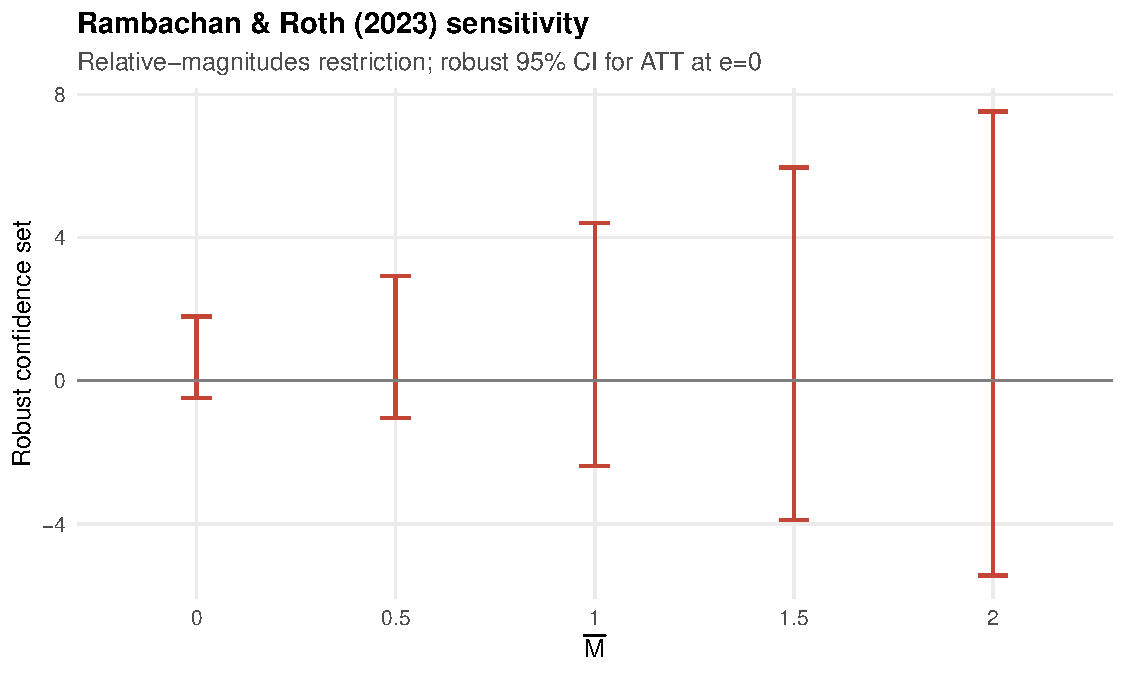
\includegraphics[width=0.8\textwidth]{fig9_honestdid.pdf}
\caption{Rambachan--Roth sensitivity. Under modest departures from parallel trends, the robust
confidence set for the post-adoption effect spans zero.}
\label{fig:honest}
\end{figure}

\paragraph{It is indistinguishable from chance.} As a final check I reassign adoption at random
among the never-treated controls, three hundred times, and re-estimate. If the true effect were
real, the observed estimate should sit in the tail of this placebo distribution. It does not: a
quarter of random placebos produce an estimate at least as large in magnitude
(Figure~\ref{fig:placebo}). The observed $+2.73$ is an ordinary draw from a distribution generated
by countries that never adopted anything.

\begin{figure}[t]
\centering
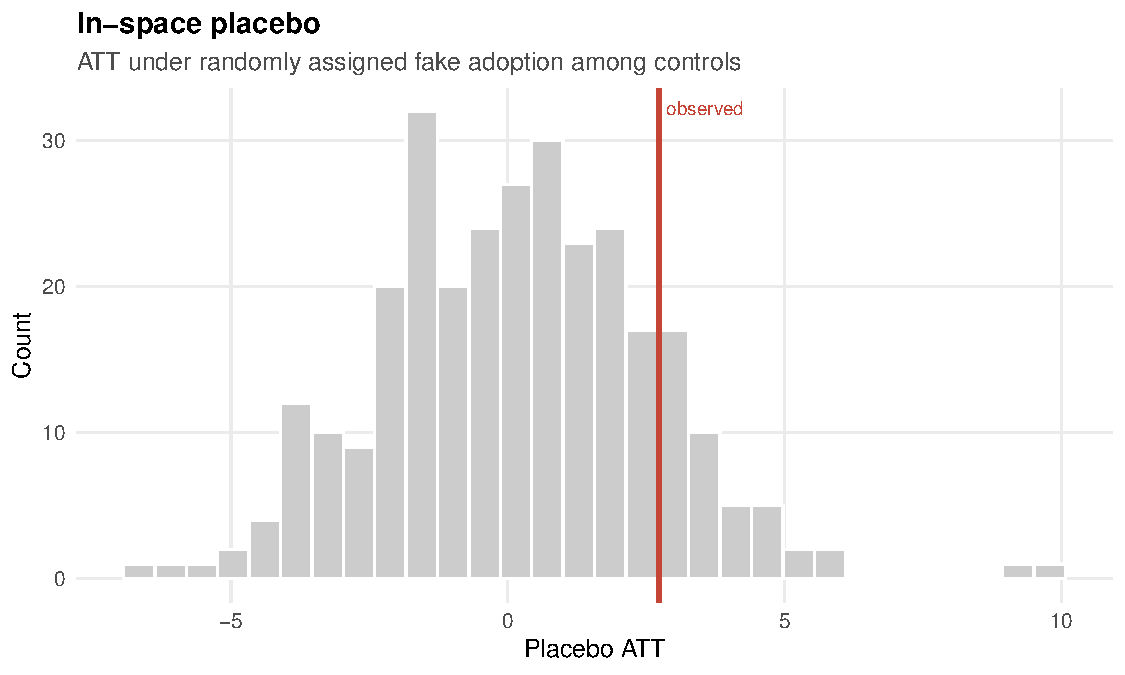
\includegraphics[width=0.8\textwidth]{fig_falsification_placebo.pdf}
\caption{In-space placebo. The observed estimate (red line) is unremarkable against effects
estimated from randomly assigned fake adoption among controls ($p = 0.25$).}
\label{fig:placebo}
\end{figure}

\paragraph{Synthetic control agrees, where it can speak at all.} The method built for a handful of
treated units \citep{abadie2010synthetic,benmichael2021augmented} can be applied only to the two
countries with enough pre-adoption history to construct a credible counterfactual---the United
Kingdom and Ireland; Norway and Sweden, with a single pre-period each, defeat it entirely, which is
itself a comment on how little the data contain. For both the UK and Ireland the augmented
synthetic control reproduces the pre-adoption path well and then drifts above it after adoption,
but the post-adoption gap is statistically ordinary: placebo $p$-values of $0.46$ and $0.69$
against control units treated as if they had adopted (Appendix~B, Figures~\ref{fig:synthUK}
and~\ref{fig:synthIE}). Ireland's gap, the larger of the two, opens in 2008. Even the method of last
resort returns the same verdict.

\paragraph{It is fragile where it should be solid.} A genuine treatment effect should not depend on
which untreated countries one happens to compare against. This one does. Dropping the four
post-communist controls---Czechia, Estonia, Hungary, Slovenia, whose suicide rates were falling
steeply from post-transition peaks throughout the window---nearly halves the estimate, to $+1.24$
(standard error $0.76$). Recoding Sweden's adoption to its 2008 parliamentary strategy leaves
$+2.41$; allowing a year of anticipation leaves $+1.68$. The sign survives; the magnitude wanders
with the specification, in the manner of an estimate that is measuring the comparison rather than
the policy.

Five windows, one answer. They are not independent of one another, but they fail together, and a
result that survives none of them is not a result. The cross-national mortality record cannot tell
us what national suicide-prevention strategies do.

\section{The Arithmetic of Governing in the Dark}

It is tempting, having demolished an estimate, to feel that something has been accomplished. Very
little has. The world's suicides are not reduced by a confidence interval, and a country deciding
tomorrow whether to write a strategy gains nothing from being told that the last twenty years of
evidence were not what they seemed---unless that knowledge changes what it does next. So let me say
what I think it should change.

It should change our confidence, not our conduct. The finding here is not that strategies are
useless; it is that the observational cross-section is structurally incapable of revealing their
worth, because countries adopt them in response to the very trends that would otherwise be used to
identify their effect, and because the post-adoption years of the principal European adopters were
swallowed by a recession that raised suicide everywhere. A policy can be both worth keeping and
unproven, and intellectual honesty requires holding those two facts at once. What is not defensible
is the laundering of association into causation that the field has practiced---the citing of a
single pre-Goodman-Bacon comparison as though it settled the matter, the diffusion of a policy on
the strength of evidence that evaporates the moment it is examined with the tools the rest of
applied economics now considers mandatory.

It should also change how we invest in knowing. The reason we cannot answer the question is not
that suicide is mysterious; it is that we adopted a continent's worth of strategies without once
building the variation that would let us evaluate them. We have no staggered randomization, no
phased regional rollout with administrative mortality data, no pre-registered evaluation attached
to a single one of these national plans. Every country switched at once, at the level at which the
confounders also live, in response to the outcome itself. If the European Commission wishes to know
whether its mental-health investments save lives---and it should wish to know, because the
alternative is to keep spending moral and fiscal capital on faith---then the evaluation must be
designed before the policy is deployed, at a level finer than the nation, with the counterfactual
built in rather than reconstructed afterward from a panel too small and too confounded to bear it.

I began with a number---one death every forty seconds---and I want to end with it, because it is
the only number in this paper that is not in dispute. The strategies were written for that number.
Whether they have moved it, I cannot tell you, and neither, I think, can anyone who looks honestly
at the cross-national data. That should not comfort the skeptic or the believer. It should frighten
both. We are making life-and-death policy in a darkness we have mistaken for evidence, and the
first step out of it is to admit that the light we thought we had was never there.

\clearpage
\appendix
\singlespacing

\section{Appendix A: Data Construction and Treatment Coding}

\paragraph{Outcome.} Eurostat table \texttt{hlth\_cd\_asdr}, age-standardized death rate for
intentional self-harm (ICD-10 X60--X84, Y87.0), sex total, per 100{,}000, 1994--2010
\citep{eurostat_cod}. The regional table \texttt{hlth\_cd\_asdr2} (NUTS-2, 2011--2023) is not used
for estimation because it postdates the adoption wave, but it confirms the national series in its
overlap.

\paragraph{Treatment.} A country is coded treated in the first year its government adopted a
stand-alone national suicide-prevention strategy, following the inclusion criterion of the WHO's
2018 inventory \citep{who2018strategies} and the peer-reviewed dates of
\citet{lewitzka2019national}. In-window adopters: Norway 1995, Sweden 1995, United Kingdom 2002
(England's national strategy; Eurostat reports the UK in aggregate), Ireland 2005. Finland (1992) is
dropped as already-treated at the panel's start; France (2000) is dropped because its outcome series
begins in 2001, leaving no pre-period. Documented never-adopters used as controls include Germany,
Italy, Spain, Belgium, Austria, Switzerland, the Netherlands, Portugal, Greece, Luxembourg, Czechia,
Estonia, Hungary, and Slovenia; the balanced sample retains the twelve with complete outcome and
covariate records (Belgium, Denmark, Italy, Poland, and Slovakia are dropped for gaps in the
suicide series). The sign of the estimate survives recoding Sweden's adoption to its 2008
parliamentary strategy ($+2.41$) and permitting one year of anticipation ($+1.68$), but its
magnitude nearly halves when the four post-communist controls are dropped ($+1.24$, s.e.\ $0.76$).
Denmark cannot be recoded as a 1998 adopter, contrary to what one might wish to test, because its
suicide series is incomplete and it does not appear in the balanced panel; and adding real GDP per
capita as a second covariate cannot be estimated at all, because the GDP-complete subsample is too
small to support it---a limitation worth stating plainly rather than burying, and itself a measure
of how little identifying information the data contain.

\paragraph{Covariate.} National unemployment rate, World Bank modeled-ILO series
\texttt{SL.UEM.TOTL.ZS}, 1994--2010 \citep{worldbank_unemp}. Real GDP per capita and population age
structure (Eurostat) are used in supplementary specifications.

\paragraph{Balance.} Table~\ref{tab:balance} reports baseline (1994) means and the standardized
difference in means---$(\bar x_T - \bar x_C)/\sqrt{(s_T^2 + s_C^2)/2}$---which
\citet{imbens2015causal} call ``imbalanced'' beyond $0.25$ in absolute value. Every comparable
covariate clears that bar. Unemployment, the covariate I condition on, is imbalanced at $0.33$:
the treated countries were not on the same cyclical footing as the controls, which is precisely why
conditioning on it is necessary rather than cosmetic. The treated countries also begin with
\emph{much lower} suicide ($-0.99$) and an older age structure---a reminder that the cross-sectional
contrast is uninformative and only the within-country trend comparison can be.

\begin{table}[h]
\centering\small
\caption{Baseline (1994) balance, treated vs.\ never-treated. Standardized difference $>0.25$ in
absolute value is ``imbalanced'' \citep{imbens2015causal}.}
\label{tab:balance}
\begin{tabular}{lcccc}
\toprule
Variable & Treated mean & Control mean & Std.\ diff. & Imbalanced? \\
\midrule
Suicide rate (per 100k) & $12.13$ & $21.53$ & $-0.99$ & yes \\
Unemployment rate (\%) & $9.78$ & $8.18$ & $+0.33$ & yes \\
Share aged 65+ (\%) & $15.23$ & $13.95$ & $+0.63$ & yes \\
Median age (years) & $35.20$ & $36.24$ & $-0.42$ & yes \\
\bottomrule
\end{tabular}
\end{table}

\paragraph{Reproducibility.} All estimates were computed independently in R (\texttt{did},
\texttt{didimputation}, \texttt{fixest}, \texttt{HonestDiD}, \texttt{augsynth}), Python
(\texttt{differences}), and Stata (\texttt{csdid}). Sample sizes and means are identical across
languages; the primary ATT replicates to four to six significant figures within matched
specifications. The cross-language replication report is archived with the paper.

\section{Appendix B: Estimators, Synthetic Control, and Additional Robustness}

\paragraph{Estimators.} The primary estimates use \citet{callaway2021did} with regression
adjustment and the never-treated comparison group, aggregated to the group-size-weighted ATT and to
event time. \citet{borusyak2024revisiting} provides the imputation estimator and its long-horizon
event study; \citet{sun2021estimating} provides the interaction-weighted estimator with
never-treated as the reference cohort. \citet{goodmanbacon2021did} and
\citet{dechaisemartin2020twoway} motivate the abandonment of two-way fixed effects;
\citet{rambachan2023credible} provides the sensitivity analysis. Doubly robust and
inverse-propensity variants \citep{santanna2020doubly} are reported but, given the absence of
common support documented in Figure~\ref{fig:pscore}, are not preferred.

\paragraph{Augmented synthetic control.} For the United Kingdom and Ireland I estimate a
ridge-augmented synthetic control \citep{abadie2010synthetic,benmichael2021augmented} against the
pool of never-treated donors, with placebo inference based on reassigning treatment to each donor
in turn and ranking the post-to-pre RMSPE ratio. Figures~\ref{fig:synthUK} and~\ref{fig:synthIE}
show the fit and the placebo distribution; the post-adoption gaps are statistically ordinary
($p=0.46$ for the UK, $p=0.69$ for Ireland) and, for Ireland, open with the 2008 recession. Norway
and Sweden cannot be analyzed by synthetic control: with a single pre-treatment year each, no
counterfactual can be constructed, which is itself a measure of how little identifying variation the
1995 cohort contains.

\begin{figure}[h]
\centering
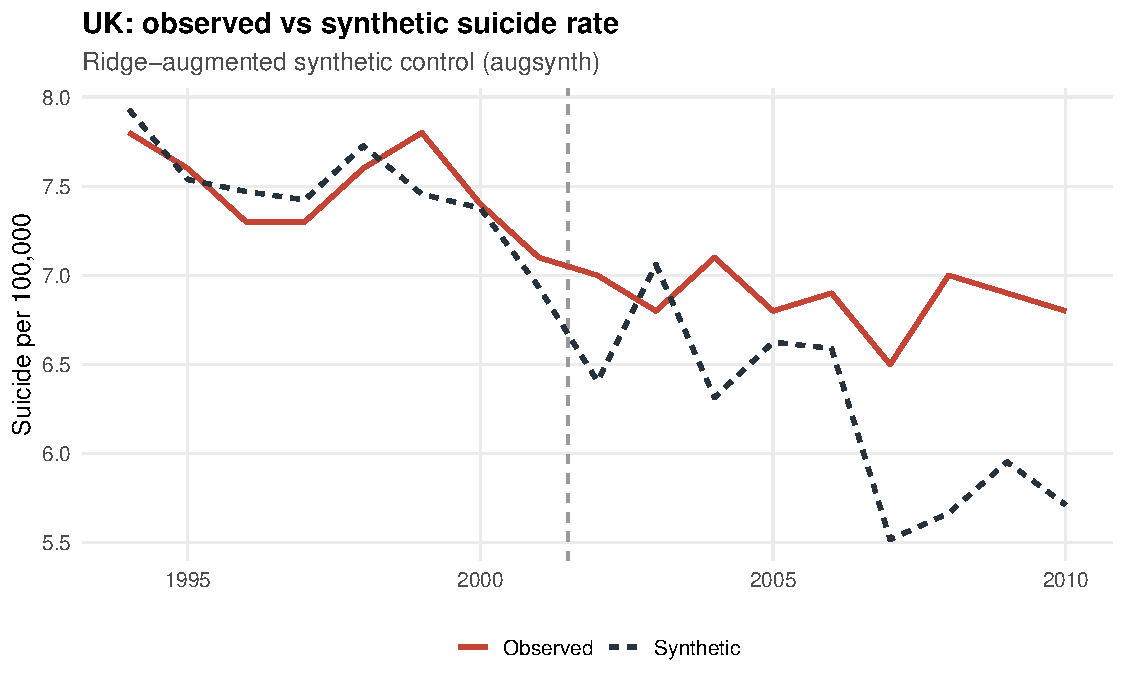
\includegraphics[width=0.49\textwidth]{fig_synth_fit_UK.pdf}
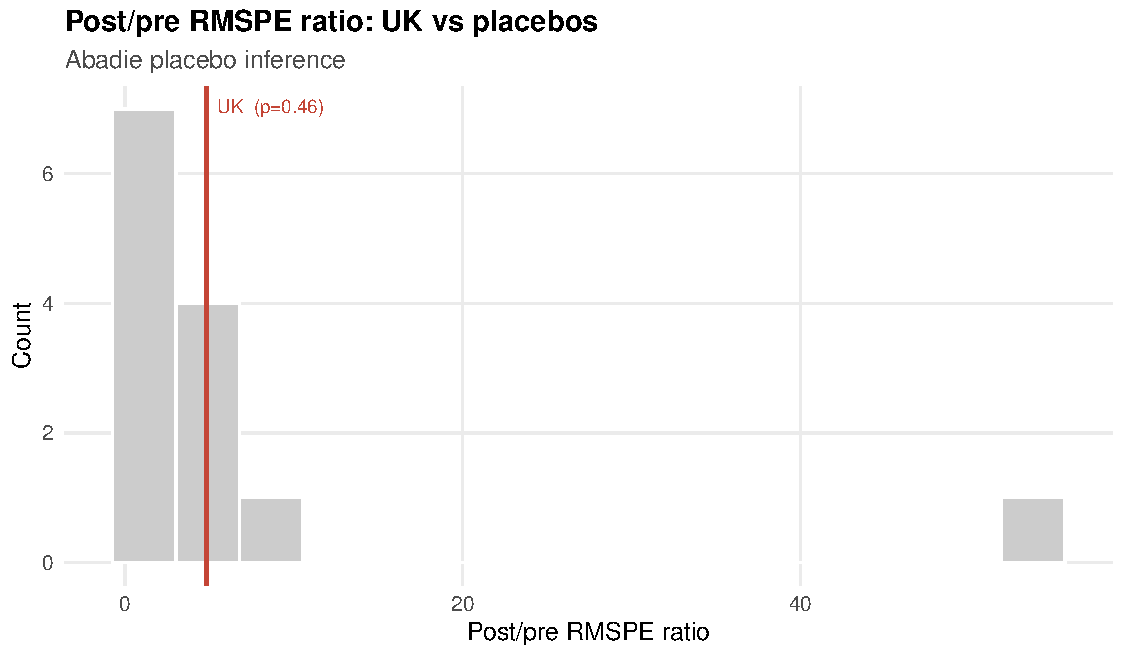
\includegraphics[width=0.49\textwidth]{fig_synth_rmspe_UK.pdf}
\caption{United Kingdom. Left: observed vs.\ synthetic suicide rate. Right: post/pre RMSPE ratio
against control placebos ($p=0.46$).}
\label{fig:synthUK}
\end{figure}

\begin{figure}[h]
\centering
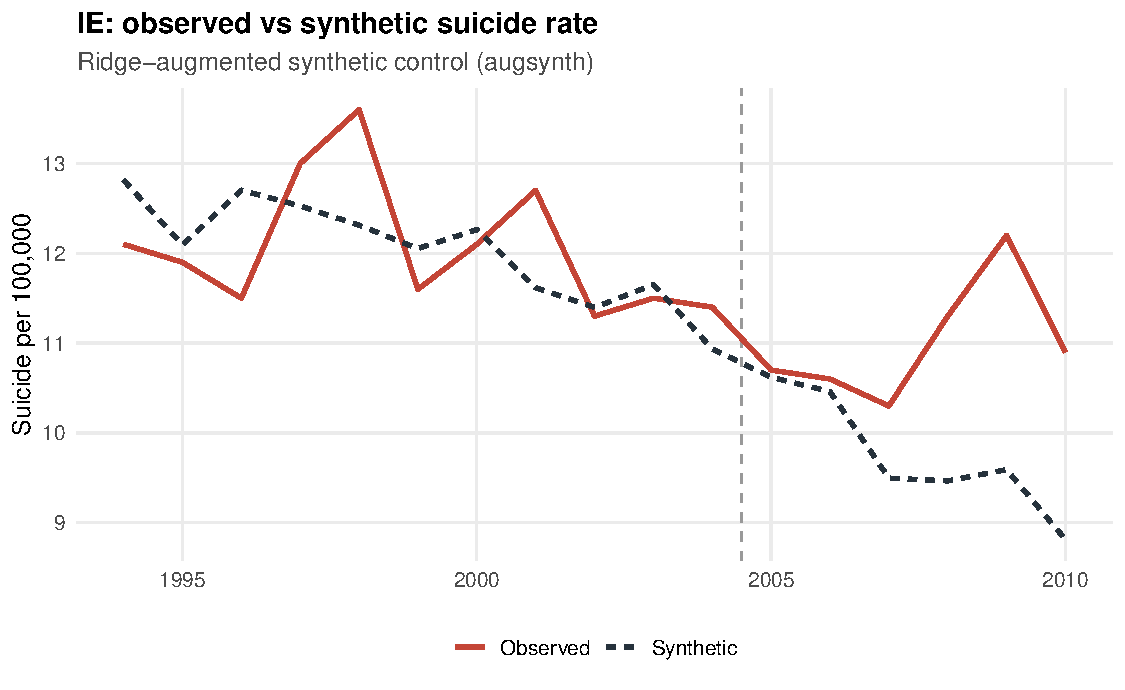
\includegraphics[width=0.49\textwidth]{fig_synth_fit_IE.pdf}
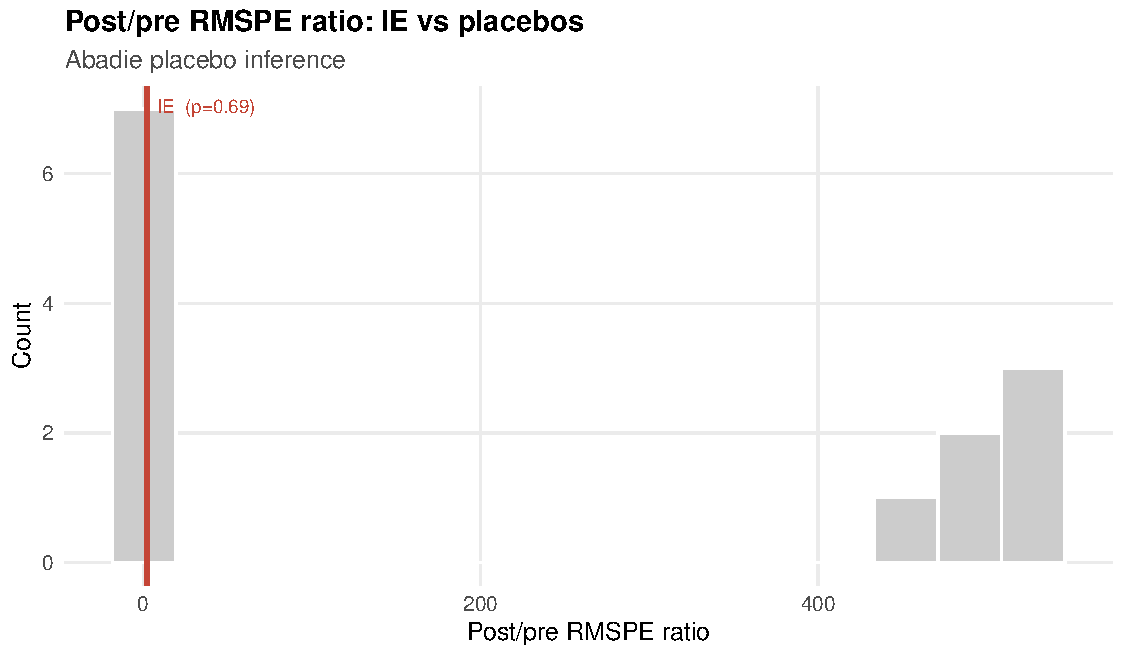
\includegraphics[width=0.49\textwidth]{fig_synth_rmspe_IE.pdf}
\caption{Ireland. Left: observed vs.\ synthetic suicide rate; the gap opens in 2008. Right: post/pre
RMSPE ratio against control placebos ($p=0.69$).}
\label{fig:synthIE}
\end{figure}

\paragraph{Leave-one-out.} Dropping each treated country in turn leaves the sign and rough
magnitude of the aggregate ATT unchanged; no single country drives the result, which is to say that
the positive estimate is a feature of the whole confounded comparison and not an artifact of one
outlier.

\paragraph{Is the two-way fixed-effects estimate the culprit?} It is fair to ask whether the whole
exercise is an artifact of the well-known pathology of two-way fixed effects under staggered
adoption \citep{goodmanbacon2021did,dechaisemartin2020twoway}. It is not. Running the static TWFE
regression of suicide on a post-adoption indicator returns a coefficient of $3.11$, and the
Goodman-Bacon decomposition (Table~\ref{tab:bacon}) reconstructs it exactly as a weighted average of
its $2\times2$ building blocks. The ``forbidden'' comparisons that use already-treated countries as
controls---the source of the bias---carry only about three percent of the total weight, because the
never-treated pool is large. The clean treated-versus-untreated comparisons carry the rest. TWFE
($3.11$) therefore sits right beside the heterogeneity-robust Callaway--Sant'Anna estimate
($2.73$): the estimator is not the problem. The problem is identification, and it is shared by every
estimator in this paper.

\begin{table}[h]
\centering\small
\caption{Goodman-Bacon decomposition of the TWFE estimate}
\label{tab:bacon}
\begin{tabular}{lccc}
\toprule
$2\times2$ comparison & Weight & Avg.\ estimate & Contribution \\
\midrule
Treated vs.\ untreated & $0.864$ & $3.57$ & $3.085$ \\
Later vs.\ earlier treated & $0.112$ & $0.29$ & $0.032$ \\
Earlier vs.\ later treated & $0.025$ & $-0.22$ & $-0.005$ \\
\midrule
Reconstructed TWFE & $1.000$ & & $3.112$ \\
\bottomrule
\end{tabular}
\end{table}

\clearpage
\singlespacing
\bibliography{references}

\end{document}
